% !TeX program = pdflatex
\documentclass{article}

% Use the preprint mode to disable anonymity (course submission).
% (The "final" mode in this template expects an internal track name.)
\usepackage[preprint]{neurips_2025}

\usepackage[utf8]{inputenc}
\usepackage[T1]{fontenc}
\usepackage{hyperref}
\usepackage{url}
\usepackage{booktabs}
\usepackage{amsfonts}
\usepackage{amssymb}
\usepackage{nicefrac}
\usepackage{microtype}
\usepackage{xcolor}
\usepackage{amsmath}
\usepackage{algorithm}
\usepackage{algorithmic}
\usepackage{graphicx}
\usepackage{tikz}
\usepackage{pgfplots}
\pgfplotsset{compat=1.18}
\usepackage{placeins}
\usepackage{float}

\newcommand{\insertdata}[1]{\textcolor{red}{[INSERT #1]}}
% To avoid accidentally including stale/incorrect generated numbers, we do not
% include auto-generated tables by default. Set \usegeneratedtrue to enable.
\newif\ifusegenerated
\usegeneratedfalse
% The course requires a strict 4-page main body. Appendix is optional.
\newif\ifuseappendix
\useappendixtrue

\title{Efficient KV Cache Management for Long-Context LLM Inference:\\ Lazy Pruning for Practical StreamingLLM}

% Course assignment submission (non-anonymous).
\author{%
  Jifan Lin (523030910057) \\
  Shanghai Jiao Tong University \\
  \texttt{ljf2570@sjtu.edu.cn} \\
  \And
  Second Author Name (XXXXXXXXXXXXX) \\
  Shanghai Jiao Tong University \\
  \texttt{email2@sjtu.edu.cn} \\
}

\begin{document}

\maketitle

\begin{abstract}
Long-context LLM inference is bottlenecked by KV-cache growth and per-token runtime overhead. StreamingLLM~\cite{xiao2023streamingllm} bounds KV-cache size by retaining attention sinks and a recent-token window, but practical decoding can still suffer from \emph{non-trivial cache-management overhead}, especially for RoPE models where pruning changes cache positions and requires positional consistency. We implement a modular StreamingLLM stack on HuggingFace (Cache API) and propose \textbf{Lazy Pruning}: a training-free strategy that batches Start+Recent compaction and RoPE re-alignment, amortizing expensive cache slicing/copy/rotation across multiple decode steps. On PG19 (20k tokens, Auto-cap 2048), Lazy Pruning improves TPOT from 19.57ms (strict Start+Recent) to 14.37ms and achieves 6.81$\times$ speedup over a sliding-window recompute baseline; its PPL increases from 19.761 to 20.318 (+2.82\% vs recompute, +0.68\% vs strict Start+Recent). Additional negative results are summarized in Appendix.
\end{abstract}

\section{Introduction}
Long-context LLM inference is challenging because both computation and memory scale with the context length. During autoregressive decoding, the KV cache grows linearly with the number of processed tokens, increasing attention cost and memory traffic. StreamingLLM~\cite{xiao2023streamingllm} mitigates this by keeping only (i) the first $S$ ``sink'' tokens and (ii) a sliding window of the most recent $W$ tokens, thereby bounding the effective KV-cache length.

\paragraph{Motivation.}
In our setting (Pythia-2.8B on NVIDIA A800), once attention length is bounded, decode becomes dominated by MLP and framework/launch overhead. Meanwhile, KV pruning itself can incur additional overhead due to slicing/copy and rotary-position re-alignment. More importantly, periodic hard eviction introduces distribution shifts that manifest as token-level NLL spikes and perplexity (PPL) degradation on long-form datasets. These observations motivate a KV-management mechanism that reduces amortized pruning overhead without modifying attention kernels or model weights.

\paragraph{Contributions.}
We make three contributions centered on a \emph{practical} StreamingLLM implementation and an amortization mechanism:
(i) we implement StreamingLLM on top of HuggingFace's Cache API while keeping attention modules unmodified, and explicitly handle RoPE consistency as a cache-side operation for plug-and-play comparisons;
(ii) we propose \textbf{Lazy Pruning}, which batches Start+Recent compaction and RoPE re-alignment to reduce amortized cache-management overhead in batch-1 decode;
(iii) we provide a reproducible pipeline and a detailed exploration log of negative results, clarifying which optimizations do or do not transfer to batch-1 streaming decode.

\section{Related Work}
\label{sec:related}
\textbf{Long-context inference and KV-cache compression.}
Test-time KV-cache management is a widely used approach to make long-context inference feasible, including retention/eviction heuristics and cache compression~\cite{xiao2023streamingllm,zhang2023h2o,liu2023scissorhands,kwon2023paged}. Our work builds on StreamingLLM's Start+Recent rule and focuses on \emph{training-free} extensions that target the practical costs of pruning and eviction-induced distribution shifts.
\textbf{Kernel- and decoding-level accelerations.}
Attention kernels such as FlashAttention aim to reduce attention IO cost~\cite{dao2022flashattention,dao2023flashattention2}, while speculative decoding accelerates generation by drafting tokens~\cite{leviathan2023speculative,chen2023accelerating}. Post-training quantization reduces compute/memory but its benefits depend on hardware and runtime regime~\cite{dettmers2022llmint8,frantar2023gptq}. We empirically find these do not improve batch-1 streaming decode in our setting and analyze the underlying reasons (Sec.~\ref{sec:negative}).

\section{Method}
\label{sec:method}
We first define Start+Recent streaming and our cache-side RoPE re-alignment, then formalize Lazy Pruning. Additional exploratory mechanisms are summarized in Appendix.

\subsection{Preliminaries: Start+Recent StreamingLLM}
Let $x_{1:t}$ be the processed prefix at decode step $t$. For each layer $\ell$, let $(\mathbf{K}_t^\ell,\mathbf{V}_t^\ell)$ denote the KV cache with sequence length $L_t$ along the cache dimension. Start+Recent streaming retains (i) the first $S$ sink tokens, and (ii) the most recent $W$ tokens. Define the soft capacity
\begin{equation}
  C_0 \triangleq S + W.
\end{equation}
Our code also supports optional \emph{non-core} retained tokens (e.g., overlap/refresh); we denote their total budget by $B\ge 0$ and define the effective soft capacity
\begin{equation}
  C \triangleq C_0 + B.
\end{equation}
Unless stated otherwise, we use $B=0$ in paper experiments to isolate Lazy Pruning.
\paragraph{Auto-cap (fixed total context budget).}
To avoid confounds from changing the \emph{total} number of visible tokens, and to respect the model's maximum context length, we adopt an \textbf{Auto-cap} protocol in our evaluation.
We fix a global cap $C_{\text{cap}}$ (e.g., $2048$ for Pythia-2.8B) and count all components that increase the visible KV length into the same budget:
\begin{equation}
S + W + \sigma + O + B \;\le\; C_{\text{cap}},
\end{equation}
where $\sigma$ is an optional slack budget (used only in exploratory experiments), $O$ is overlap (if enabled), and $B$ is the refresh budget.
Equivalently, for a fixed $C_{\text{cap}}$ we derive the recent-window size as
\begin{equation}
W \;=\; C_{\text{cap}} - S - \sigma - O - B.
\end{equation}
This defines the post-prune \emph{target length} and prevents methods from silently seeing more tokens when enabling slack/overlap/refresh, making speed--quality comparisons reproducible. Under strict Start+Recent pruning ($R{=}1$), the cache is kept at $C_{\text{cap}}$ every step. Under Lazy Pruning with interval $R$, the cache is still pruned back to $C_{\text{cap}}$, but can temporarily overflow between prunes; in our implementation the peak cache length during a forward pass is bounded by $C_{\text{cap}}+R$ (Fig.~\ref{fig:kvlen}).
\paragraph{Peak-length bound (fairness).}
Because pruning is applied \emph{after} each forward pass, the effective attention length during forward can exceed the post-prune target. For a given pruning interval $R$, the forward-time cache length satisfies:
\begin{equation}
  L_t^{\text{fwd}} \le C_{\text{cap}} + R.
\end{equation}
We report speed and quality under a fixed post-prune target $C_{\text{cap}}$, and provide an overhead breakdown (Appendix~\ref{tab:profile_prune}) to attribute speedups to amortized cache-management overhead rather than attention-length effects.
When pruning is performed, the retained index set is
\begin{equation}
  \mathcal{I}_t \;=\; \{0,1,\ldots,S-1\}\;\cup\;\{L_t-W,\ldots,L_t-1\},
\end{equation}
with the recent segment clamped to avoid overlap with the sink segment.

\paragraph{RoPE consistency.}
For rotary-position-embedding models (e.g., Pythia/GPT-NeoX), pruning changes token positions in the cache; therefore, cached keys must be re-aligned to the new positions. We implement RoPE consistency as a cache-side operation (without modifying attention forwards); the derivation and implementation details are deferred to Appendix~\ref{app:rope}.

\subsection{Lazy Pruning}
Na\"ive streaming prunes as soon as the cache exceeds $C$, which can add overhead due to slicing/copy and KV relocation. We instead amortize pruning by triggering compaction only when overflow reaches a threshold $R$ (in code: \texttt{compress\_every}), reducing the frequency of expensive prune+RoPE re-alignment operations.
Define overflow:
\begin{equation}
  \mathrm{overflow}_t \triangleq L_t - C.
\end{equation}
Let $R$ be the \emph{pruning interval/allowance} hyperparameter (in code: \texttt{compress\_every}). In bounded-memory evaluation we use $R\ge 1$. Lazy pruning triggers only when overflow reaches $R$:
\begin{equation}
  \mathrm{PruneTrigger}(t) \triangleq \mathbb{1}\big[\mathrm{overflow}_t \ge R\big].
\end{equation}
This choice explicitly trades a slightly larger instantaneous cache length for fewer expensive prune-and-realign events, which is effective when pruning overhead is non-negligible under batch-1 decode. Fig.~\ref{fig:kvlen} illustrates the resulting sawtooth behavior. For debugging, our code also supports disabling pruning via \texttt{compress\_every=0}; we do not use this mode in bounded-memory comparisons.
\begin{figure}[t]
\centering
% Auto-generated by experiments/paper/generate_fig1_kv_length.py
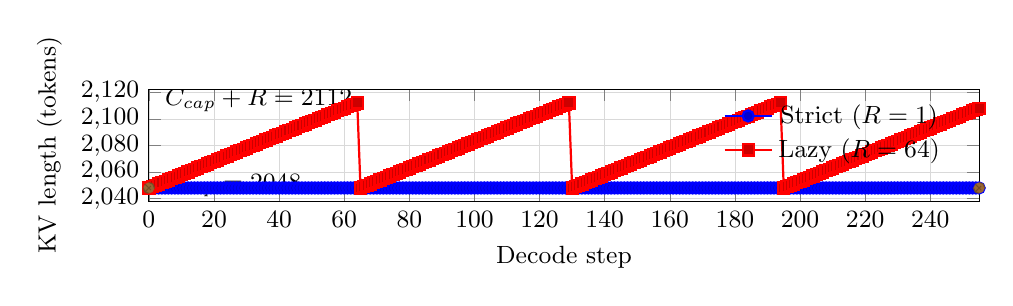
\begin{tikzpicture}
\begin{axis}[
    width=\linewidth,
    height=3.0cm,
    xlabel={Decode step},
    ylabel={KV length (tokens)},
    xmin=0, xmax=255,
    ymin=2038, ymax=2122,
    grid=both,
    grid style={line width=.1pt, draw=gray!20},
    major grid style={line width=.2pt,draw=gray!30},
    legend style={draw=none, fill=none, font=\small},
    legend pos=north east,
    tick label style={font=\small},
    label style={font=\small},
]
\addplot+[thick] coordinates { (0,2048) (1,2048) (2,2048) (3,2048) (4,2048) (5,2048) (6,2048) (7,2048) (8,2048) (9,2048) (10,2048) (11,2048) (12,2048) (13,2048) (14,2048) (15,2048) (16,2048) (17,2048) (18,2048) (19,2048) (20,2048) (21,2048) (22,2048) (23,2048) (24,2048) (25,2048) (26,2048) (27,2048) (28,2048) (29,2048) (30,2048) (31,2048) (32,2048) (33,2048) (34,2048) (35,2048) (36,2048) (37,2048) (38,2048) (39,2048) (40,2048) (41,2048) (42,2048) (43,2048) (44,2048) (45,2048) (46,2048) (47,2048) (48,2048) (49,2048) (50,2048) (51,2048) (52,2048) (53,2048) (54,2048) (55,2048) (56,2048) (57,2048) (58,2048) (59,2048) (60,2048) (61,2048) (62,2048) (63,2048) (64,2048) (65,2048) (66,2048) (67,2048) (68,2048) (69,2048) (70,2048) (71,2048) (72,2048) (73,2048) (74,2048) (75,2048) (76,2048) (77,2048) (78,2048) (79,2048) (80,2048) (81,2048) (82,2048) (83,2048) (84,2048) (85,2048) (86,2048) (87,2048) (88,2048) (89,2048) (90,2048) (91,2048) (92,2048) (93,2048) (94,2048) (95,2048) (96,2048) (97,2048) (98,2048) (99,2048) (100,2048) (101,2048) (102,2048) (103,2048) (104,2048) (105,2048) (106,2048) (107,2048) (108,2048) (109,2048) (110,2048) (111,2048) (112,2048) (113,2048) (114,2048) (115,2048) (116,2048) (117,2048) (118,2048) (119,2048) (120,2048) (121,2048) (122,2048) (123,2048) (124,2048) (125,2048) (126,2048) (127,2048) (128,2048) (129,2048) (130,2048) (131,2048) (132,2048) (133,2048) (134,2048) (135,2048) (136,2048) (137,2048) (138,2048) (139,2048) (140,2048) (141,2048) (142,2048) (143,2048) (144,2048) (145,2048) (146,2048) (147,2048) (148,2048) (149,2048) (150,2048) (151,2048) (152,2048) (153,2048) (154,2048) (155,2048) (156,2048) (157,2048) (158,2048) (159,2048) (160,2048) (161,2048) (162,2048) (163,2048) (164,2048) (165,2048) (166,2048) (167,2048) (168,2048) (169,2048) (170,2048) (171,2048) (172,2048) (173,2048) (174,2048) (175,2048) (176,2048) (177,2048) (178,2048) (179,2048) (180,2048) (181,2048) (182,2048) (183,2048) (184,2048) (185,2048) (186,2048) (187,2048) (188,2048) (189,2048) (190,2048) (191,2048) (192,2048) (193,2048) (194,2048) (195,2048) (196,2048) (197,2048) (198,2048) (199,2048) (200,2048) (201,2048) (202,2048) (203,2048) (204,2048) (205,2048) (206,2048) (207,2048) (208,2048) (209,2048) (210,2048) (211,2048) (212,2048) (213,2048) (214,2048) (215,2048) (216,2048) (217,2048) (218,2048) (219,2048) (220,2048) (221,2048) (222,2048) (223,2048) (224,2048) (225,2048) (226,2048) (227,2048) (228,2048) (229,2048) (230,2048) (231,2048) (232,2048) (233,2048) (234,2048) (235,2048) (236,2048) (237,2048) (238,2048) (239,2048) (240,2048) (241,2048) (242,2048) (243,2048) (244,2048) (245,2048) (246,2048) (247,2048) (248,2048) (249,2048) (250,2048) (251,2048) (252,2048) (253,2048) (254,2048) (255,2048) };
\addlegendentry{Strict ($R=1$)}
\addplot+[thick] coordinates { (0,2048) (1,2049) (2,2050) (3,2051) (4,2052) (5,2053) (6,2054) (7,2055) (8,2056) (9,2057) (10,2058) (11,2059) (12,2060) (13,2061) (14,2062) (15,2063) (16,2064) (17,2065) (18,2066) (19,2067) (20,2068) (21,2069) (22,2070) (23,2071) (24,2072) (25,2073) (26,2074) (27,2075) (28,2076) (29,2077) (30,2078) (31,2079) (32,2080) (33,2081) (34,2082) (35,2083) (36,2084) (37,2085) (38,2086) (39,2087) (40,2088) (41,2089) (42,2090) (43,2091) (44,2092) (45,2093) (46,2094) (47,2095) (48,2096) (49,2097) (50,2098) (51,2099) (52,2100) (53,2101) (54,2102) (55,2103) (56,2104) (57,2105) (58,2106) (59,2107) (60,2108) (61,2109) (62,2110) (63,2111) (64,2112) (65,2048) (66,2049) (67,2050) (68,2051) (69,2052) (70,2053) (71,2054) (72,2055) (73,2056) (74,2057) (75,2058) (76,2059) (77,2060) (78,2061) (79,2062) (80,2063) (81,2064) (82,2065) (83,2066) (84,2067) (85,2068) (86,2069) (87,2070) (88,2071) (89,2072) (90,2073) (91,2074) (92,2075) (93,2076) (94,2077) (95,2078) (96,2079) (97,2080) (98,2081) (99,2082) (100,2083) (101,2084) (102,2085) (103,2086) (104,2087) (105,2088) (106,2089) (107,2090) (108,2091) (109,2092) (110,2093) (111,2094) (112,2095) (113,2096) (114,2097) (115,2098) (116,2099) (117,2100) (118,2101) (119,2102) (120,2103) (121,2104) (122,2105) (123,2106) (124,2107) (125,2108) (126,2109) (127,2110) (128,2111) (129,2112) (130,2048) (131,2049) (132,2050) (133,2051) (134,2052) (135,2053) (136,2054) (137,2055) (138,2056) (139,2057) (140,2058) (141,2059) (142,2060) (143,2061) (144,2062) (145,2063) (146,2064) (147,2065) (148,2066) (149,2067) (150,2068) (151,2069) (152,2070) (153,2071) (154,2072) (155,2073) (156,2074) (157,2075) (158,2076) (159,2077) (160,2078) (161,2079) (162,2080) (163,2081) (164,2082) (165,2083) (166,2084) (167,2085) (168,2086) (169,2087) (170,2088) (171,2089) (172,2090) (173,2091) (174,2092) (175,2093) (176,2094) (177,2095) (178,2096) (179,2097) (180,2098) (181,2099) (182,2100) (183,2101) (184,2102) (185,2103) (186,2104) (187,2105) (188,2106) (189,2107) (190,2108) (191,2109) (192,2110) (193,2111) (194,2112) (195,2048) (196,2049) (197,2050) (198,2051) (199,2052) (200,2053) (201,2054) (202,2055) (203,2056) (204,2057) (205,2058) (206,2059) (207,2060) (208,2061) (209,2062) (210,2063) (211,2064) (212,2065) (213,2066) (214,2067) (215,2068) (216,2069) (217,2070) (218,2071) (219,2072) (220,2073) (221,2074) (222,2075) (223,2076) (224,2077) (225,2078) (226,2079) (227,2080) (228,2081) (229,2082) (230,2083) (231,2084) (232,2085) (233,2086) (234,2087) (235,2088) (236,2089) (237,2090) (238,2091) (239,2092) (240,2093) (241,2094) (242,2095) (243,2096) (244,2097) (245,2098) (246,2099) (247,2100) (248,2101) (249,2102) (250,2103) (251,2104) (252,2105) (253,2106) (254,2107) (255,2108) };
\addlegendentry{Lazy ($R=64$)}
\addplot+[dashed] coordinates { (0,2048) (255,2048) };
\node[anchor=west, font=\small] at (axis cs:2,2050) {$C_{cap}=2048$};
\node[anchor=west, font=\small] at (axis cs:2,2114) {$C_{cap}+R=2112$};
\end{axis}
\end{tikzpicture}

\caption{KV-cache length during decoding under Auto-cap. Strict Start+Recent ($R{=}1$) prunes every step and stays at $C_{\text{cap}}$. Lazy Pruning ($R{=}64$) reduces prune frequency at the cost of bounded oscillation; the peak forward-time length is bounded by $C_{\text{cap}}+R$. KV length is proportional to KV memory footprint and influences the amount of cache compaction work.}
\label{fig:kvlen}
\end{figure}

\paragraph{Rule form.}
Strict pruning (Start+Recent) prunes whenever $\mathrm{overflow}_t>0$. Lazy Pruning prunes only when $\mathrm{overflow}_t\ge R$, then compacts back to $C$ and re-aligns RoPE (Appendix~\ref{app:rope}).

\section{Experiments}
\label{sec:exp}

\subsection{Setup}
We evaluate on Pythia-2.8B. We use WikiText-103 as a short-context sanity check and PG19 as the primary long-context benchmark~\cite{pg19}. Due to space, the main paper focuses on TPOT, speedup over recompute, PPL, and peak GPU memory; additional metrics are logged by our evaluator.
\textbf{Datasets.} We use WikiText-103~\cite{merity2016pointer} and PG19~\cite{pg19}.
\textbf{Baselines and fairness.}
We compare methods under the same fixed soft cap $C_{\text{cap}}$ (Auto-cap; Sec.~\ref{sec:method}). The non-streaming baseline uses a sliding window of length $C_{\text{cap}}$ and recomputes attention each step (no KV cache), while StreamingLLM variants reuse KV cache and apply pruning/re-alignment targeting a post-prune length of $C_{\text{cap}}$; Lazy Pruning may temporarily overflow between prunes but remains bounded.
All methods share the same model, dataset segment, and evaluation protocol implemented in \texttt{experiments/eval\_streaming\_llm.py}.

\paragraph{Protocol.}
We use a fixed evaluation protocol implemented in \texttt{experiments/eval\_streaming\_llm.py} and report TPOT, speedup over recompute, PPL, and peak GPU memory.

\subsection{Main Results and Ablations}
\paragraph{Comparison protocol.}
We compare a strict Start+Recent baseline (immediate pruning, $R{=}1$) against our Lazy Pruning variant (batched pruning, $R{>}1$) under a fixed KV budget (Auto-cap, $S{+}W{=}2048$). This isolates the effect of pruning frequency and cache-management overhead under the same bounded-attention regime.
\ifusegenerated
  \IfFileExists{generated/tables.tex}{\begin{table}[H]
\centering
\caption{Main results on PG19 (long-context) under Auto-cap $C_{\text{cap}}{=}2048$.}
\small
\begin{tabular}{lcccc}
\toprule
Method & TPOT$\downarrow$ & Speedup$\uparrow$ & PPL$\downarrow$ & Peak Mem (MB)$\downarrow$ \\
\midrule
Baseline (Sliding Window, no KV) & 97.91 & 1.00$\times$ & 19.761 & 5723 \\
StreamingLLM (Start+Recent; strict prune) & 19.57 & 5.00$\times$ & 20.181 & 6941 \\
Ours (Lazy Pruning) & 14.37 & 6.81$\times$ & 20.318 & 6941 \\
\bottomrule
\end{tabular}
\end{table}

\begin{table}[H]
\centering
\caption{Sanity-check results on WikiText-103 (short-context).}
\small
\begin{tabular}{lccc}
\toprule
Method & TPOT$\downarrow$ & Speedup$\uparrow$ & PPL$\downarrow$ \\
\midrule
Baseline (Sliding Window, no KV) & 97.36 & 1.00$\times$ & 9.359 \\
StreamingLLM (Start+Recent; strict prune) & 20.22 & 4.79$\times$ & 9.496 \\
Ours (Lazy Pruning) & 14.45 & 6.68$\times$ & 9.519 \\
\bottomrule
\end{tabular}
\end{table}
}{}
\else
  \begin{table}[t]
  \centering
  \caption{Main results on PG19 (long-context) under Auto-cap $C_{\text{cap}}{=}2048$.}
  \small
  \begin{tabular}{lcccc}
  \toprule
  Method & TPOT$\downarrow$ & Speedup$\uparrow$ & PPL$\downarrow$ & Peak Mem (MB)$\downarrow$ \\
	  \midrule
	  Baseline (Sliding Window, no KV) & 97.91 & 1.00$\times$ & 19.761 & 5723 \\
	  StreamingLLM (Start+Recent; strict prune) & 19.57 & 5.00$\times$ & 20.181 & 6941 \\
	  Ours (Lazy Pruning; $R{=}64$) & 14.37 & 6.81$\times$ & 20.318 & 6941 \\
	  \bottomrule
	  \end{tabular}
	  \end{table}
\fi
\paragraph{Main finding.}
On PG19 under the same Auto-cap budget, Lazy Pruning reduces TPOT from 19.57ms (strict Start+Recent, $R{=}1$) to 14.37ms ($R{=}64$), a further 1.36$\times$ improvement over strict pruning, with a small additional PPL increase (20.181 $\rightarrow$ 20.318) and unchanged peak memory in our evaluator.
\textbf{Evidence for amortization.} Under a controlled PG19 probe where only $R$ changes, the forward-time component stays nearly constant while cache-update overhead drops sharply as prune events become infrequent, consistent with a simple decomposition $\mathrm{TPOT}\approx T_{\text{fwd}} + T_{\text{update}}/R$ (Appendix~\ref{tab:profile_prune}).
\paragraph{Fairness and measurement notes.}
Auto-cap fixes the post-prune target length to $C_{\text{cap}}{=}2048$, while Lazy Pruning allows bounded overflow between prunes with peak forward-time length $C_{\text{cap}}{+}R$. Peak GPU memory is measured as \texttt{torch.cuda.max\_memory\_allocated()} in our evaluator; the additional KV introduced by $R{=}64$ is small relative to total memory and may not change the rounded peak value.

\paragraph{Ablations.}
We report the full ablation ladder, additional $R$ settings, and exploratory quality heuristics (Slack/Max\_Drop, overlap/refresh) in Appendix~\ref{app:full-results}. In the main body we focus on the strict ($R{=}1$) vs lazy ($R{=}64$) contrast as the primary effect.

\section{Discussion}
\label{sec:negative}
\paragraph{Bottleneck shift: forward dominates after cache management is amortized.}
After StreamingLLM bounds the attention length and Lazy Pruning amortizes prune+RoPE re-alignment overhead, most remaining runtime concentrates in the model forward pass. We evaluated several standard accelerations (FlashAttention, speculative decoding, quantization, \texttt{torch.compile}/CUDA Graphs, StaticCache, and a CUDA micro-kernel), but none provided consistent net gains in our batch-1 long-context streaming regime (Appendix~\ref{app:neg}).

\section{Conclusion}
We present a practical StreamingLLM implementation on HuggingFace and a single effective optimization: Lazy Pruning, which amortizes Start+Recent compaction and RoPE re-alignment overhead in batch-1 streaming decode. On PG19, Lazy Pruning achieves 6.81$\times$ speedup over a sliding-window recompute baseline (vs 5.00$\times$ for strict Start+Recent) under a fixed context budget with minor PPL degradation (+2.82\% vs recompute, +0.68\% vs strict).

\ifuseappendix
  \clearpage
  \FloatBarrier
  \appendix
  \renewcommand{\thetable}{A\arabic{table}}
  \setcounter{table}{0}
  \section{Appendix}
  \FloatBarrier

  \subsection{Limitations and future work}
  Our results suggest that in a bounded-attention, batch-1 decoding regime, end-to-end latency quickly becomes forward dominated once KV length is capped and cache-update costs are amortized. In this regime, Lazy Pruning yields a measurable TPOT reduction with only a small additional PPL increase under a fixed post-prune target length.
  However, our approach has several limitations. (i) The remaining speed bottleneck is the model forward pass (GEMMs and associated pointwise/LN ops); further gains likely require kernel- or graph-level optimization beyond cache management. (ii) Lazy Pruning permits bounded overflow ($C_{\text{cap}}{+}R$ peak forward-time length), and our peak-memory reporting uses \texttt{torch.cuda.max\_memory\_allocated()}, which can be insensitive to small KV differences at MB granularity; repeated runs and finer-grained reporting (allocated vs reserved; mean$\pm$std) are needed. (iii) We observe a small PPL increase relative to strict Start+Recent and did not find consistently beneficial quality-oriented heuristics under Auto-cap, indicating that improving quality without regressing speed may require different cache-consistency mechanisms.
  Future work includes: (i) cache layouts with static/ring-buffer semantics to better support compilation/graph capture; (ii) fused transformer-block implementations or alternative backends to reduce forward overhead; and (iii) broader evaluation across models, longer contexts, and multiple runs to quantify variance and robustness.

  \subsection{Implementation notes and pseudocode}
  \label{app:impl}
  We summarize the core pruning rule (Start+Recent) and our Lazy Pruning trigger ($R$) in Algorithm~\ref{alg:kv}. This pseudocode matches the implementation setting used in our evaluator (Auto-cap, prune-to-$C_{\text{cap}}$).

  \begin{algorithm}[h]
  \caption{KV pruning with Lazy Pruning (implementation-level summary)}
  \label{alg:kv}
  \small
  \begin{algorithmic}[1]
  \REQUIRE sink size $S$, window size $W$, extra budget $B$ (default 0), pruning interval $R\ge 1$
   \STATE $C \leftarrow S+W+B$
   \STATE observe cache length $L_t$
   \IF{$L_t \le C$} \STATE \textbf{return} \ENDIF
   \IF{$L_t - C < R$} \STATE \textbf{return} \ENDIF
   \STATE keep first $S$ tokens and most recent $(C - S)$ tokens
   \STATE prune KV cache and re-align RoPE positions
  \end{algorithmic}
  \end{algorithm}

  \subsection{RoPE consistency derivation}
  \label{app:rope}
  For rotary-position-embedding models, pruning changes token positions in the cache; therefore cached keys must be re-aligned to the new positions.
  Let $p$ be an old token position and $p'$ its new position after compaction. RoPE encodes position via per-dimension frequencies $\omega_i$ (from \texttt{inv\_freq}). Re-alignment is equivalent to a delta rotation with $\Delta p = p'-p$:
  \begin{equation}
  \begin{bmatrix}
  k'_{2i}\\k'_{2i+1}
  \end{bmatrix}
  =
  \begin{bmatrix}
  \cos(\omega_i \Delta p) & -\sin(\omega_i \Delta p)\\
  \sin(\omega_i \Delta p) & \cos(\omega_i \Delta p)
  \end{bmatrix}
  \begin{bmatrix}
  k_{2i}\\k_{2i+1}
  \end{bmatrix}.
  \end{equation}
  In the Start+Recent setting, the recent block undergoes a constant position shift, enabling reuse of rotation factors across layers.

\subsection{Full experimental results}
\label{app:full-results}
  % Do not repeat the main-table numbers here; we only include additional
  % sanity checks and breakdowns.
  \IfFileExists{generated/wikitext_sanity.tex}{\begin{table}[H]
\centering
\caption{Sanity-check results on WikiText-103 (short-context).}
\small
\begin{tabular}{lccc}
\toprule
Method & TPOT$\downarrow$ & Speedup$\uparrow$ & PPL$\downarrow$ \\
\midrule
Baseline (Sliding Window, no KV) & 97.36 & 1.00$\times$ & 9.359 \\
StreamingLLM (Start+Recent; strict prune) & 20.22 & 4.82$\times$ & 9.496 \\
Ours (Lazy Pruning) & 14.45 & 6.74$\times$ & 9.519 \\
\bottomrule
\end{tabular}
\end{table}
}{}
  \IfFileExists{generated/profile_prune_overhead.tex}{\begin{table}[H]
\centering
\caption{Profiling evidence for amortization (PG19 probe; fixed $C_{\text{cap}}=2048$, $S=32$, $\sigma=16$): forward time stays nearly constant while cache-update overhead is amortized by increasing $R$.}
\label{tab:profile_prune}
\small
\begin{tabular}{lcccc}
\toprule
Setting & Prune events & Forward (ms) & Update (ms) & Total (ms) \\
\midrule
Strict ($R=1$) & 2000 & 14.12 & 5.57 & 19.69 \\
Lazy ($R=64$) & 31 & 14.03 & 0.09 & 14.12 \\
\bottomrule
\end{tabular}
\end{table}
}{}
  \IfFileExists{generated/ablations.tex}{\begin{table}[H]
\centering
\caption{Ablation ladder on PG19 (aligned $S,W$). Differences below \textasciitilde1\% may fall within run-to-run noise unless stated otherwise.}
\small
\begin{tabular}{lccc}
\toprule
Setting & TPOT$\downarrow$ & Speedup$\uparrow$ & PPL$\downarrow$ \\
\midrule
Start+Recent (strict prune) ($R{=}1$) & 19.57 & 5.00$\times$ & 20.181 \\
Start+Recent (strict prune; framework-only) ($R{=}1$) & 20.02 & 4.89$\times$ & 20.181 \\
+ Lazy Pruning ($R{=}64$) & 14.38 & 6.80$\times$ & 20.318 \\
+ (expl.) Slack ($R{=}64$, $\sigma{=}16$) & 14.35 & 6.82$\times$ & 20.262 \\
+ (expl.) Slack + Max\_Drop ($R{=}64$, $\sigma{=}16$, $\delta{=}32$) & 14.53 & 6.74$\times$ & 20.272 \\
\bottomrule
\end{tabular}
\end{table}
}{}

  \subsection{Negative results (evidence-backed)}
  \label{app:neg}
  \IfFileExists{generated/negative_results.tex}{\begin{table}[H]
\centering
\caption{Summary of investigated but ineffective optimization routes in our batch-1 streaming setting.}
\small
\begin{tabular}{p{0.34\linewidth}p{0.18\linewidth}p{0.40\linewidth}}
\toprule
Method & Outcome & Notes (see project logs) \\
\midrule
FlashAttention / FlashDecoding & Inconclusive / low ROI & Integration is sensitive to environment and attention implementation; once streaming bounds attention length, speed is often dominated by MLP and launch/framework overhead. \\
Speculative decoding & Negative result & In long-context workloads, draft/target mismatch yields low acceptance rates, making SpecDec slower than normal decoding. \\
Quantization (TorchAO INT8/INT4) & Slower / unstable & INT8 WO v1 produced NaNs; v2 is stable but slower for batch-1 decode in our stack; INT4 backend dependencies were problematic. \\
\texttt{torch.compile} / CUDA Graphs & Unstable & Repeated-run CUDA graph overwrite errors observed in rotary-embedding path; shape/cache semantics hinder capture. \\
HF StaticCache & Incompatible & StaticCache assumes fixed cache updates; pruning can trigger device-side asserts (index out of bounds). \\
CUDA fusion (residual/LN) & Slower & Amdahl's law: residual/LN is a small fraction; custom kernel launch overhead dominated (0.92$\times$, TPOT +8.6\%). \\
\bottomrule
\end{tabular}
\end{table}
}{}

  \paragraph{Speculative decoding in long-context workloads.}
  We evaluated speculative decoding with small/medium draft models in a long-context PG19 workload. While a \emph{draft=target} sanity check achieved near-perfect acceptance, using smaller drafts led to low acceptance rates and poor tokens-per-target-forward, making speculative decoding slower than normal decoding. We attribute this to draft/target distribution mismatch at long positions.

  \paragraph{FlashAttention integration.}
  We prepared an evaluation path that can switch attention backends (math/SDPA/FlashAttention when available). In our regime, streaming already bounds attention length, so overall speed is often dominated by MLP and framework/launch overhead; additionally, FlashAttention availability depends on GPU/driver/toolchain, making it difficult to include as a stable default in the reproducible mainline.

  \paragraph{Fused CUDA residual add.}
  We implemented and rigorously validated a fused CUDA residual-add kernel for GPT-NeoX (bit-exact hidden states and generation outputs), but it was slower (0.92$\times$, TPOT +8.6\%), consistent with Amdahl's law and kernel-launch dominated micro-ops.

  \paragraph{MIT reference implementation notes.}
  The MIT StreamingLLM reference repo applies \texttt{pos\_shift} patches inside model attention forwards, while our implementation preserves HuggingFace attention modules and performs RoPE consistency as cache-side operations. Under our Transformers version, we observed that the MIT long-PPL script did not produce consistent metrics for GPT-NeoX; therefore we avoid drawing quality claims from cross-codebase PPL and focus on within-evaluator comparisons.
\fi

\bibliographystyle{plainnat}
\bibliography{references}

\end{document}
